\documentclass[aspectratio=169]{beamer}

%---------------------------
%       Beamer Cheat Sheet
%---------------------------
% https://www.cpt.univ-mrs.fr/~masson/latex/Beamer-appearance-cheat-sheet.pdf

%---------------------------
%       Set Theme and Colors
%---------------------------

\usetheme[width=.1\paperwidth]{Hannover}
% \setbeamertemplate{sidebar canvas right}[vertical shading][top=red,bottom=blue]

\definecolor{QESblue}{HTML}{8AD2ED}
\definecolor{QESdarkblue}{HTML}{187ca2}
\definecolor{QESlightblue}{HTML}{c4e8f6}

\setbeamercolor{sidebar}{bg=QESlightblue}
\setbeamercolor{titlelike}{fg=QESdarkblue}

\setbeamercolor{palette sidebar secondary}{fg=QESdarkblue}
\setbeamercolor{title in sidebar}{fg=QESdarkblue}
\setbeamercolor{author in sidebar}{fg=QESdarkblue}

\addtobeamertemplate{sidebar left}{}{\vfill \hspace{.006\paperwidth} 
\includegraphics[width=.08\paperwidth]{../../../logo.png} \vspace{.006\paperwidth} } 
% \addtobeamertemplate{sidebar left}{}{\vfill \hspace{.00001\paperwidth} 
\includegraphics[width=.093\paperwidth]{../../figures/qes-qr.png} \vspace{.003\paperwidth} } 

%---------------------------
%       No navigation symbols
%---------------------------
\setbeamertemplate{navigation symbols}{}

%---------------------------
%       Set Fonts
%---------------------------
\usepackage{helvet}
\renewcommand{\familydefault}{\sfdefault}
\usepackage{sansmathfonts}
\usepackage{upgreek}

\setbeamerfont{frametitle}{series=\bfseries, size=\Large}
\setbeamerfont{title in sidebar}{series=\bfseries, size=\small}
\setbeamertemplate{caption}{\it\raggedright\insertcaption\par}

%---------------------------
%       Math font packages
%---------------------------
\usepackage{dsfont, amsmath, amsthm, mathtools}
\usepackage{bbm, bm}
\usepackage[T1]{fontenc}
\usepackage[version=3]{mhchem}

%---------------------------
%       Figure packages
%---------------------------
\usepackage{graphicx}
\graphicspath{{../../figures}}

\usepackage{epstopdf}
\usepackage{color}

\setbeamerfont{caption}{size=\footnotesize}

\usepackage{subfigure}

%---------------------------
%       Manual placement packages
%---------------------------
\usepackage{tikz}
\usetikzlibrary{calc}

%---------------------------
%       Local Macros
%---------------------------

\newcommand{\manualpic}[4]{
    % inputs {filename}{figure options}{x offset}{y offset}
    \tikz[remember picture, overlay] \node[anchor=center] at ($(current page.center)+(#3,#4)$) {\includegraphics[#2]{#1}};
}

\newcommand{\manualtext}[3]{
    % inputs {text}{x offset}{y offset}
    \tikz[remember picture, overlay] \node[anchor=center] at ($(current page.center)+(#2,#3)$) {#1};
}

\newcommand{\manualtextleft}[3]{
    % inputs {text}{x offset}{y offset}
    \tikz[remember picture, overlay] \node[anchor=west] at ($(current page.center)+(#2,#3)$) {#1};
}

\newcommand{\manualtextright}[3]{
    % inputs {text}{x offset}{y offset}
    \tikz[remember picture, overlay] \node[anchor=east] at ($(current page.center)+(#2,#3)$) {#1};
}

\newcommand{\slidereference}[1]{
    \manualtextleft{\tiny #1}{-0.47\linewidth}{-0.47\textheight}
}

\newcommand{\dv}[2]{\frac{\mathrm{d}#1}{\mathrm{d}#2}}

\title{Ocean Carbon}
\author{2/5}

\begin{document}

\begin{frame}{The Solubility Pump}

\end{frame}

\section{Patterns}

\begin{frame}{Patterns of Ocean Carbon}
    \centering
    \slidereference{Sarmiento \& Gruber (2006)}

    \includegraphics<1>[width=\linewidth, totalheight=0.75\textheight, keepaspectratio]{carbon-cx-dic.png}

    \includegraphics<2>[width=\linewidth, totalheight=0.75\textheight, keepaspectratio]{carbon-ocean-atmos.png}

\end{frame}

\section{Dissolution}

\begin{frame}{\ce{CO2} dissolves in water}
    \centering
    \ce{[CO2]} = $\mathbf{K_0}$ \ce{pCO2}

    \onslide<2>{
        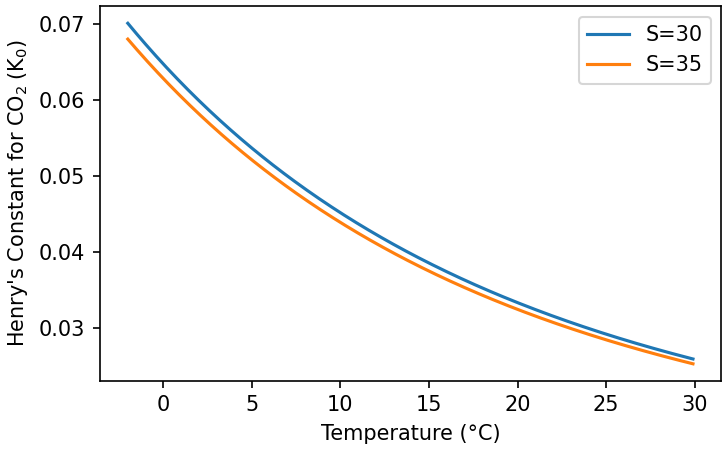
\includegraphics[width=\linewidth, totalheight=0.65\textheight, keepaspectratio]{carbon_K0.png}
    }

\end{frame}

\begin{frame}{\ce{CO2} dissolves in water}
    \centering
    
    \includegraphics<1>[width=\linewidth, totalheight=0.7\textheight, keepaspectratio]{sst-month.png}

    \includegraphics<2>[width=\linewidth, totalheight=0.7\textheight, keepaspectratio]{ocean-heat-flux.png}

    \manualpic{carbon_K0.png}{width=3cm}{-0.36\linewidth}{0.39\textheight}

\end{frame}

\section{Solubility Pump}

\begin{frame}{The Solubility Pump}
    \centering

    \only<2-5>{
        \manualpic{carbon_K0.png}{width=3cm}{-0.36\linewidth}{0.39\textheight}
    }

    \includegraphics<1>[width=\linewidth, totalheight=0.65\textheight, keepaspectratio]{carbon-circ-surface.png}

    \includegraphics<2>[width=\linewidth, totalheight=0.65\textheight, keepaspectratio]{carbon-circ-TS.png}

    \includegraphics<3>[width=\linewidth, totalheight=0.65\textheight, keepaspectratio]{carbon-circ-TS-Cin.png}

    \includegraphics<4>[width=\linewidth, totalheight=0.65\textheight, keepaspectratio]{carbon-circ-TS-DIC.png}

    \includegraphics<5>[width=\linewidth, totalheight=0.65\textheight, keepaspectratio]{carbon-circ-solubility.png}

    \includegraphics<6>[width=\linewidth, totalheight=0.75\textheight, keepaspectratio]{carbon-ocean-atmos.png}

    \includegraphics<7>[width=\linewidth, totalheight=0.75\textheight, keepaspectratio]{carbon-cx-dic.png}

\end{frame}

\begin{frame}{The Solubility Pump}
\begin{itemize}
    \item Explains first-order surface \ce{\Delta pCO2} patterns.
    \item Explains relative enrichment of C in the deep ocean.
    \item \textbf{Doesn't} explain high concentration of C in the ocean\dots
    \item \textbf{Doesn't} explain increasing deep C concentration along circulation path\dots
\end{itemize}

\end{frame}


\section{Reaction}

\begin{frame}{\ce{CO2} reacts with water}

    \only<1->{
        \manualtextleft{\ce{CO2 + H2O \Leftrightarrow H2CO3}}{-6cm}{2cm}
        \manualpic{carbon-CO2.png}{height=1.1cm}{-5.5cm}{3cm}
        \manualpic{carbon-H2O.png}{height=1.1cm}{-4.5cm}{3cm}

        \manualpic{carbon-H2CO3.png}{height=2cm}{-2.1cm}{0.7cm}    
    }
    
    \only<2->{
        \manualtextleft{\ce{H2CO3 \Leftrightarrow H^+ + HCO3^-}}{-1.8cm}{0cm}
        \manualpic{carbon-HCO3.png}{height=1.8cm}{2cm}{-1.2cm}
    }

    \only<3->{
        \manualtextleft{\ce{HCO3^- \Leftrightarrow H^+ + CO3^{2-}}}{1.8cm}{-2.5cm}
        \manualpic{carbon-CO3.png}{height=1.8cm}{6.3cm}{-3.5cm}
    }

\end{frame}

\begin{frame}{\ce{CO2} reacts with water}

    \centering
    \onslide<1->{
        $
        \mathrm{CO_{2(g)} \Leftrightarrow \underbrace{CO_{2(aq)}}_{dissolved~gas} + H_2O \Leftrightarrow \underbrace{H_2CO_3}_{carbonic~acid} \Leftrightarrow \underbrace{HCO_3^-}_{bicarbonate} + H^+ \Leftrightarrow \underbrace{CO_3^{2-}}_{carbonate} + 2H^+}
        $
    }

    \onslide<2->{    
        \bigskip
        \bigskip
        $ \mathrm{DIC = [CO_{2(aq)}] + [H_2CO_3] + [HCO_3^-] + [CO_3^{2-}]} $
    }


\end{frame}

\begin{frame}{\ce{CO2} reacts with water}

    \centering
    $
    \mathrm{CO_{2(g)} \Leftrightarrow \underbrace{\mathbf{[CO_2^*]}}_{dissolved~gas} \Leftrightarrow \underbrace{HCO_3^-}_{bicarbonate} + H^+ \Leftrightarrow \underbrace{CO_3^{2-}}_{carbonate} + 2H^+}
    $

    \bigskip
    \bigskip
    $ \mathrm{DIC = \mathbf{[CO_2^*]} + [HCO_3^-] + [CO_3^{2-}]} $

\end{frame}


\section{Speciation}

\begin{frame}{DIC Speciation}

    \centering
    \includegraphics<1>[width=\linewidth, totalheight=0.65\textheight, keepaspectratio]{carbon_bjerrum.png}

\end{frame}

\begin{frame}{DIC Speciation}
\centering
$ \mathrm{DIC = [CO_2^*] + [HCO_3^-] + [CO_3^{2-}]} $
\bigskip\bigskip

\begin{tabular}{ccl}
    $\mathrm{CO_2^* \xLeftrightarrow{K_1} HCO_3^- + H^+}$ && $K_1 = \mathrm{\frac{[H^+][HCO_3^-]}{[CO_2^*]}}$ \\
    \bigskip && \\
    $\mathrm{HCO_3^- \xLeftrightarrow{K_2} CO_3^{2-} + H^+}$ && $K_2 = \mathrm{\frac{[H^+][CO_3^{2-}]}{[HCO_3^-]}}$ \\
\end{tabular}

\onslide<2>{
    \bigskip\bigskip
    $ \mathrm{[CO_2^*] = \frac{DIC}{1 + \frac{K_1}{[H^+]} + \frac{K_1K_2}{[H^+]^2}}} $
}

\end{frame}

% DIC allows ocean to take up more carbon


\section{DIC, \ce{pCO2} \& pH}

% K sensitivity to T & S 
% variable DOC/CO2, depends on starting state & physical conditions
% Ocean Acidification

\begin{frame}{DIC Speciation}

\end{frame}

\section{Modelling Solubility}

\begin{frame}{Modelling the Solubility Pump}

\begin{enumerate}
    \item Add a box to represent the atmosphere.
    \item Parameterise the exchange of \ce{CO2} between the atmosphere and the surface ocean.
    \item Track the speciation of DIC in the surface ocean.
    \item Track the concentration of DIC.
\end{enumerate}

\end{frame}

\end{document}


% \begin{frame}{TITLE}
% \end{frame}